\documentclass[a4paper, twocolumn, 11pt]{beamer}

%\usetheme{Darmstadt}
\usetheme{Warsaw}
\usefonttheme[onlylarge]{structurebold}
\setbeamerfont*{frametitle}{size=\normalsize,series=\bfseries}
%\setbeamertemplate{navigation symbols}{}

\usepackage[cp1250]{inputenc}
\usepackage[english]{babel}
\usepackage{times}
\usepackage[T1]{fontenc}
\usepackage{pgf}
\usepackage{tikz}
\usepackage{listings}

\newcommand{\jmltobmltext}{JML2BML}
\newcommand{\jmltobml}{\textsl{\jmltobmltext}\xspace}
\newcommand{\openjml}{OpenJML\xspace}
\newcommand{\bmllib}{BMLLib\xspace}

\lstdefinelanguage{BML}{morekeywords={abstract,break,byte,case,catch,char,class,%
      const,continue,default,do,double,else,extends,false,final,%
      finally,float,for,goto,if,implements,import,instanceof,%
      interface,label,long,native,new,
      boolean, int,%
      null,%
      package,private,protected,public,ghost,%
      return,short,static,super,switch,synchronized,this,throw,%
      throws,transient,true,try,void,volatile,while,
      requires,precondition,ensures,exsures,exists,forall,&&,%
      old_this,loop_inv,\result,\everything,\nothing,%
      loop_specification,modifies,invariant,decreases,%
      iconst_0,iconst_1,istore_3,iinc,iload_3,%
      aaload,aload_0,aload_1,aload_2,aastore,%
      if_acmpne,if_icmplt,%
      invokespecial,getfield,%
      arraylength,ireturn},%
   sensitive,%
   morecomment=[l]//,%
   morestring=[b]",%
   morestring=[b]',%
    basicstyle=\scriptsize,
    keywordstyle=\bfseries\color{black},
    commentstyle=\itshape\color{blue},
    mathescape=true,
}

\title{Supplementing Java Bytecode with Specifications}
\author[Fulara, Jakubczyk, Schubert]{%
  J�drzej~Fulara \and
  Krzysztof~Jakubczyk \and
  Aleksy~Schubert \and
}
\institute{
Institute of Informatics\\
University of Warsaw\\
ul. Banacha 2\\
02-097 Warsaw, Poland
}
\date[CEE-SET 2008]{3rd IFIP TC2 Central and East European Conference on Software Engineering Techniques}

\begin{document}

\begin{frame}
\titlepage
\end{frame}

\begin{frame}{Outline}
  \tableofcontents
\end{frame}

\section{Introduction}

\subsection{Security of programs}

\begin{frame}{Problem}
  \begin{block}{We want programs to be}
    \begin{itemize}
    	\item Secure
    	\item Trustworthy
    	\item Bug-free
    \end{itemize}
  \end{block}
  \pause
  \begin{block}{Currently these are obtained by}
    \begin{itemize}
    	\item Bytecode verification
    	\item Digital certificates
    	\item Static code analysis
    	\item Runtime checking
    \end{itemize}
  \end{block}
\end{frame}

\subsection{MOBIUS project}

\begin{frame}{Idea}
	\begin{block}{Goal}
		Give the user certain guarantees of the code to be executed at the moment of its execution.
	\end{block}

	\pause

	\begin{block}{Solution}
		\alert{Proof-Carrying Code}:
		Augmented executable code with a proof that the code obeys certain policies.
	\end{block}
\end{frame}

\begin{frame}
	\frametitle{Platform - JVM bytecode}
	\begin{itemize}
		\item JVM is mature
		\item Popular (in commerce)
		\item Supports many languages \\
			\begin{itemize}
				\item Java
				\item Python (Jython)
				\item Ruby (JRuby)
				\item JavaScript (Rhino)
				\item Scala
			\end{itemize}
		\pause
	\end{itemize}
		\small{\emph{We are just going to take the 'J' off the 'JVM' and just make it a 'VM'}}\\
		\begin{flushright}		 
\footnotesize{Jonathan Schwartz,\\Sun Microsystems President and CEO}
		\end{flushright}
\end{frame}

\begin{frame}{PCC architecture for bytecode}
\begin{figure}
\begin{center}
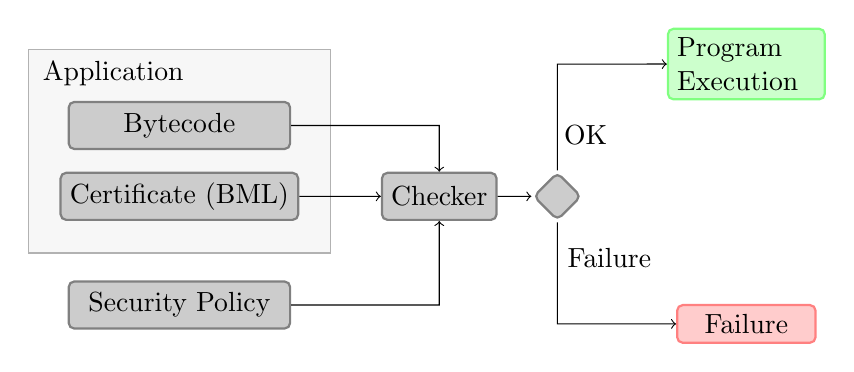
\begin{tikzpicture}[scale=0.6]

\tikzstyle{vertex}=[rectangle,draw=black!50,fill=black!20,thick,rounded corners = 2pt, minimum width=80pt, minimum height=17pt]
\tikzstyle{vertex2}=[rectangle,draw=black!50,fill=black!20,thick,rounded corners = 2pt, minimum height=17pt]
\tikzstyle{vertex3}=[rectangle,draw=green!50,fill=green!20,thick,rounded corners = 2pt, minimum width=55pt, text width=50pt]
\tikzstyle{vertex4}=[rectangle,draw=red!50,fill=red!20,thick,rounded corners = 2pt, minimum width=50pt]

\tikzstyle{rotated}=[rectangle,draw=black!50,fill=black!20,thick,rounded corners = 2pt,rotate=45, minimum height=12pt, minimum width = 12pt]
\tikzstyle{rl}=[line join = round]
\filldraw[draw=black!30,fill=black!3] (-3.2,3.8) rectangle (3.2,-0.5);
\node (app) at(-1.4,3.3) {Application};
\node[vertex] (bytecode) at (0,2.2){Bytecode};
\node[vertex] (certificate) at (0,0.7) {Certificate (BML)};

\node[vertex](policy) at (0, -1.6) {Security Policy};

\node[vertex2](checker) at (5.5,0.7) {Checker};
\node[rotated](rot) at (8, 0.7) {};
\node[vertex3](execution) at (12,3.5) {Program Execution};
\node[vertex4](failure) at (12,-2) {Failure};
\draw[->] (certificate) to[out=0,in=180] (checker);
\draw[->] (checker.east) -- (7.45,0.7);
\draw[->] (bytecode.east) -- (5.5,2.2) -- (checker.north);
\draw[->] (policy.east) -- (5.5,-1.6) -- (checker.south);
\draw[->] (8,1.25) -- (8,3.5) -- (execution.west);
\draw[->] (8,0.15) -- (8,-2) -- (failure.west);
\node (ok) at (8.6, 2) {OK};
\node (ok) at (9.1, -0.6) {Failure};
\end{tikzpicture}
\end{center}
\end{figure}
\end{frame}

\begin{frame}{PCC infrastructure}
PCC building blocks include:
\begin{itemize}
	\item construction of PCC certificates
	\item annotations in source code, languages such as JML
	\item<1->\alert<2> {compilers that transform programs to JVM bytecode with annotations}
	\item checker tools for bytecode annotations (BML) combined with PCC certificates
\end{itemize}
\end{frame}

\section{Background}

\subsection{Java Modeling Language}

\begin{frame}[fragile]
	\frametitle{What is JML?}
		Java Modeling Language (JML) features:
			\begin{itemize}
				\item behavioural specification language for Java
				\item write specifications in \emph{design-by-contract} fashion
				\item annotations written in Java comments
				\item Java syntax and semantics
			\end{itemize}
%powiedzie� kilka zda� o JMLu: �e ma sk�adni� podobn� do wyra�e� Javy, jakiego typu w�asno�ci si� w nim da wyrazi� (pre/post
%condition, niezmienniki, asserty...)
\end{frame}

\begin{frame}[fragile]
	\frametitle{JML example}

\lstset{language=java, morekeywords={requires,ensures,\result,\exists,\old,loop_invariant,\forall,==>, decreases},
        basicstyle=\tiny,commentstyle=\tiny,moredelim=*[s][\tiny]{/*@}{*/},
        numbers=left,numberstyle=\tiny,stepnumber=2,numbersep=4pt}
\begin{lstlisting}
public class List {

  private Object[] list;

  /*@ requires list != null;
    @ ensures \result ==(\exists int i;
    @                    0 <= i && i < list.length &&
    @                    \old(list[i]) == o1 && list[i] == o2);
    @*/
  public boolean replace(Object o1, Object o2){
    /*@
      @ loop_invariant i <= list.length
      @                && i >=0 && (\forall int k;0 <= k
      @                             && k < i ==> list[k] != o1);
      @ decreases list.length - i;
      @*/
    for (int i = 0; i < list.length; i++) {
      if (list[i] == o1) {
        list[i] = o2;
        return true;
      }
    }
    return false;
  }
}
\end{lstlisting}

\end{frame}

\subsection{Bytecode Modeling Language}

\begin{frame}[fragile]
	\frametitle{What is BML? [1/2]}
		Bytecode Modeling Language (BML) features:
		\begin{itemize}
			\item specification language for Java bytecode
			\item design follows fundamental concepts of JML
			\item inherits most constructions and keywords from the JML syntax
			\item BML is developed within the MOBIUS project
		\end{itemize}
\end{frame}
\begin{frame}[fragile]
	\frametitle{What is BML? [2/2]}
		Bytecode Modeling Language (BML) features:
		\begin{itemize}
			\item class files with BML annotations are regular Java class files
			\item annotations are stored within additional attributes
			\item attributes start with the prefix \emph{org.bmlspecs} and should be ignored in normal execution
			\item following the logical structure of class files: 
				\begin{itemize}
					\item class specifications are stored as class attributes
					\item method specifications are stored as method attributes 
					\item specifications inserted in the bytecode are subattributes of the JVM Code attributes.
				\end{itemize}
		\end{itemize}
\end{frame}

\begin{frame}[fragile]
	\frametitle{BML example}

\begin{figure}[htb]
\lstset{language=bml}
\lstset{basicstyle=\tiny,stepnumber=400,numbersep=5pt}
\vspace{-2\baselineskip}
~\hspace{2cm}~\begin{minipage}{400pt}
\begin{lstlisting}
/*@
  @ requires this.list != null
  @ ensures \result == (\exists int i; 0 <= i
  @                     && i < this.list.length
  @                     && old_this.list[i] == o1
  @                     && this.list[i] == o2)
  @*/
public boolean replace(Object o1, Object o2)
0:    iconst_0
1:    istore_3
...
28:   aload_0
29:   getfield	   main.List.list
32:   arraylength
/*@
  @ loop_specification
  @   modifies everything
  @   invariant i <= this.list.length
  @             && i >= 0
  @             && (\forall int k; 0 <= k
  @                 && k < i ==> this.list[k] != o1)
  @   decreases this.list.length - i
  @*/
33:   if_icmplt	   #5
36:   iconst_0
37:   ireturn
\end{lstlisting}
\end{minipage}


\label{fig:bytecode}
\end{figure}
%2:    goto	   #27
%5:    aload_0
%6:    getfield	   main.List.list
%9:    iload_3
%10:   aaload
%11:   aload_1
%12:   if_acmpne	   #24
%15:   aload_0
%16:   getfield	   main.List.list
%19:   iload_3
%20:   aload_2
%21:   aastore
%22:   iconst_1
%23:   ireturn
%24:   iinc	   %3	1
%27:   iload_3

\end{frame}

\section{JML2BML Compiler}
\subsection{Introduction}

\begin{frame}{Introduction}
	\begin{block}{Task}
		Translate JML annotations to BML annotations.
	\end{block}
	\begin{block}{Input}
		\begin{itemize}
			\item Java source file with JML annotations
			\item corresponding class file
		\end{itemize}
	\end{block}
	\begin{block}{Output}
		\begin{itemize}
			\item class file with proper BML annotations inserted
		\end{itemize}
	\end{block}
\end{frame}

\subsection{Design}

\begin{frame}{Key features}
  \begin{columns}
    \column{0.5\textwidth}
    	JML2BML compiler:
	\begin{itemize}
		\item uses OpenJml AST
		\item uses BMLLib
		\item has acyclic structure of modules
		\item uses translation rules for translating JML clauses
		\item compatible with other bytecode level tools, such as the bytecode editor Umbra
	\end{itemize}
\column{0.5\textwidth}

\tiny{
\begin{figure}[h]
  \centering{
    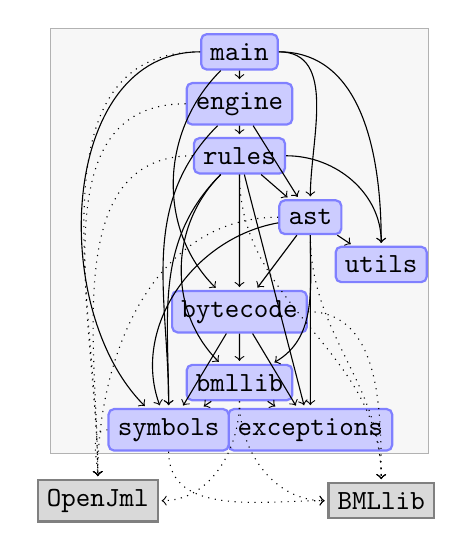
\begin{tikzpicture}[shorten >=1pt,->,scale=0.6]
      \tikzstyle{vertex}=[rectangle,draw=blue!50,fill=blue!20,thick,rounded corners = 2pt]
      \filldraw[draw=black!30,fill=black!3] (-1,7.5) rectangle (7,-1.5);
      %\draw (-0.9,7.2) node[right]{\textbf{\texttt{jml2bml}}};
      \node[vertex] (main) at (3,7) {\texttt{main}};
      \node[vertex] (engine) at (3,5.9) {\texttt{engine}}  ;
      \node[vertex] (rules) at (3,4.8) {\texttt{rules}}  ;
      \node[vertex] (ast) at (4.5,3.5) {\texttt{ast}}  ;
      \node[vertex] (utils) at (6,2.5) {\texttt{utils}};
      \node[vertex] (bytecode) at (3,1.5) {\texttt{bytecode}};
      \node[vertex] (bmllib) at (3, 0) {\texttt{bmllib}};
      \node[vertex] (exceptions) at (4.5, -1) {\texttt{exceptions}};
      \node[vertex] (symbols) at (1.5, -1) {\texttt{symbols}};
      \draw (main) -- (engine);
      \draw (engine) -- (rules);
      \draw (rules) --(ast);
      \draw (engine) -- (ast) ;
      \draw(ast) -- (utils) ;
      \draw(ast) -- (bytecode);
      \draw (ast) to[out=270,in=30] (bmllib);
      \draw (ast) -- (exceptions);
      \draw (main) to[out=0,in=90] (ast);
      \draw (rules) to[out=0,in=90] (utils);
      \draw (rules) to[out=225,in=90] (symbols);
      \draw (rules) -- (exceptions);
      \draw (rules) to[out=225,in=135] (bmllib);
      \draw (main) to[out=0,in=90] (utils);
      \draw (main) to[out=225,in=135] (bytecode);
      \draw (main) to[out=180,in=135] (symbols);
      \draw (engine) to[out=225,in=90] (symbols);
      \draw (ast) to[out=190,in=110] (symbols) ;
      \draw (rules) -- (bytecode);
      \draw (bytecode) -- (bmllib) ;
      \draw (bytecode) -- (exceptions) ;
      \draw (bytecode) -- (symbols) ;
      \draw (bmllib) -- (exceptions) ;
      \draw (bmllib) -- (symbols) ;
      \tikzstyle{external}=[rectangle,draw=black!50,fill=black!15,thick]
      \node[external] (BmlLib1) at  (6, -2.5) {\texttt{BMLlib}};
      \node[external] (openJml) at  (0, -2.5) {\texttt{OpenJml}};
      \draw[dotted] (main) to[out=180,in=90] (openJml);
      \draw[dotted] (engine) to[out=180,in=90] (openJml);
      \draw[dotted] (rules) to[out=180,in=90] (openJml);
      \draw[dotted] (rules) to[out=270,in=90] (BmlLib1);
      \draw[dotted] (ast) to[out=270,in=90] (BmlLib1);
      \draw[dotted] (ast) to[out=180,in=90] (openJml);
      \draw[dotted] (bytecode) to[out=0,in=90] (BmlLib1);
      \draw[dotted] (bmllib) to[out=270,in=0] (openJml);
      \draw[dotted] (bmllib)  to[out=270,in=180] (BmlLib1);
      \draw[dotted] (symbols) to[out=180,in=90] (openJml);
      \draw[dotted] (symbols) to[out=270,in=180] (BmlLib1);
    \end{tikzpicture}
}

\end{figure}}
\end{columns}

\end{frame}

\begin{frame}{Translation mechanism}
	\begin{block}{Translation rule}
		\begin{itemize}
	  	\item responsible for relatively small, independent piece of translation
	  	\item responsible for translation of AST subtree
	  	\item may write results of the translation to the output class file
		\end{itemize}
	\end{block}
	
  \pause
  
  \begin{block}{Features of the design}
  	\begin{itemize}
  		\item the concept falls into a visitor design pattern
  		\item translation rule is an extension of a simple abstract class
  		\item translation process can be broken into smaller, independent pieces
  		\item easily extensible
  	\end{itemize}
  \end{block}
\end{frame}

\subsection{Translating loop invariants}

\begin{frame}{Loop invariant annotations}
	\begin{block}{Where should we place annotations?}
		First instruction after loop control expression.
	\end{block}
	\begin{block}{Translation rule steps}
		\begin{itemize}
			\item detect loops in bytecode
			\item match loops from bytecode with loops from source file
			\item translate loop invariant expression
			\item attach translated expression to the right bytecode instruction.
		\end{itemize}
	\end{block}
\end{frame}

\begin{frame}{Detecting loops}
	Bytecode loop detection mechanism:
	\begin{itemize}
		\item Covers different ways of compiling loops into bytecode
\scriptsize{\centering{
\begin{tikzpicture}[shorten >=1pt,->, scale=0.7]
\tikzstyle{vertex}=[circle,draw=blue!50,fill=blue!20,thick,minimum size=13pt,inner sep=0pt]
\foreach \name/\text/\y in {s/.../1, a/a/2, b/b/3, body/.../4, c/c/5, d/d/6, e/.../7}
\node[vertex] (G-\name) at (\y,0) {$\text$};
\foreach \from/\to in {s/a,b/body,body/c,c/d,d/e}
\draw (G-\from) -- (G-\to);
\draw (G-a) to[out=45,in=135] (G-c);
\draw (G-d) to[out=225,in=315] (G-b);

\foreach \name/\text/\y in {s/.../1, a/a/2, b/b/3, body/.../4, c/c/5, d/d/6, e/.../7}
\node[vertex] (Q-\name) at (\y,-2) {$\text$};
\foreach \from/\to in {s/a,a/b,b/body, body/c, d/e}
\draw (Q-\from) -- (Q-\to);
\draw (Q-b) to[out=45,in=135] (Q-d);
\draw (Q-c) to[out=225,in=315](Q-a);

\foreach \name/\text/\x in {s/.../1, a/a/2, body1/.../3, b/b/4, body2/.../5, c/c/6, d/.../7}
\node[vertex] (X-\name) at (\x,-4) {$\text$};
\foreach \from/\to in {s/a,a/body1, body1/b, b/body2, body2/c}
\draw (X-\from) -- (X-\to);
\draw (X-b) to[out=315,in=225] (X-d);
\draw (X-c) to[out=135,in=45] (X-a);

\end{tikzpicture}
}}\normalsize
		\item Based on advanced Control Flow Graph analysis
		\item Finds entry point to the loop
	\end{itemize}
% powiedzie� o tym, do kt�rego miejsca dopisujemy anotacje. Mo�liwe pytanie: jakie s� sposoby kompilowania p�tli?
\end{frame}

\begin{frame}{Matching with source}
	Loop matching mechanism:
	\begin{itemize}
		\item uses \emph{line number table}
		\item handles \texttt{finally} block of \texttt{try-catch} statement
	\end{itemize}
\end{frame}

% \subsection{Application}
% \begin{frame}
%	zastosowanie
% \end{frame}

\section*{Summary}

\begin{frame}
  \frametitle<presentation>{TODO / In progress}
	\begin{itemize}
		\item translate JML levels higher than JML0
		\item create Eclipse plugin
		\item adapt to newer versions of BMLLib and OpenJml
		\item perform real benchmark
		\item match loops without \emph{line number table}
	\end{itemize}

\end{frame}

\end{document}
